% Two-point propagator flow

\documentclass[tikz]{standalone}

\usetikzlibrary{patterns,decorations.markings}

\tikzset{
    cross/.style={fill=white,path picture={\draw[black] (path picture bounding box.south east) -- (path picture bounding box.north west) (path picture bounding box.south west) -- (path picture bounding box.north east);}},
    dressed/.style={fill=white,postaction={pattern=north east lines}},
    momentum/.style 2 args={->,semithick,yshift=5pt,shorten >=5pt,shorten <=5pt},
    loop/.style 2 args={thick,decoration={markings,mark=at position {#1} with {\arrow{>},\node[anchor=\pgfdecoratedangle-90,font=\footnotesize] {$p_{#2}$};}},postaction={decorate}},
    label/.style={thin,gray,shorten <=-1.5ex}
}

\def\lrad{5/4}
\def\mrad{0.15*\lrad}
\def\srad{0.1*\lrad}

\begin{document}

% Diagram 1
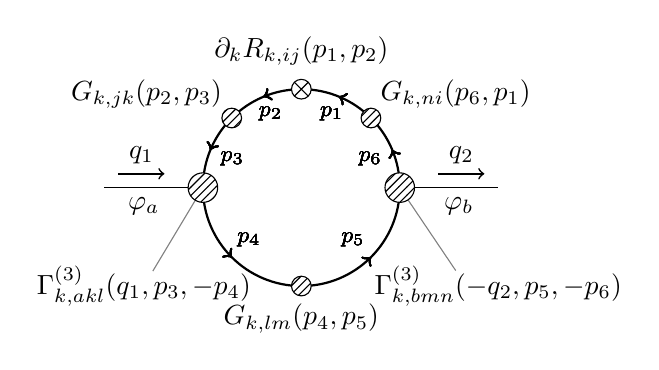
\begin{tikzpicture}
  % Loop
  \draw[loop/.list={{0.0625}{6},{0.0625*3}{1},{0.0625*5}{2},{0.0625*7}{3},{0.0625*10}{4},{0.0625*14}{5}}] (0,0) circle (\lrad);
  \draw[cross] (0,\lrad) circle (\srad) node[above=5pt] {$\partial_k R_{k,ij}(p_1,p_2)$};
  \draw[dressed] (135:\lrad) circle (\srad) node[above left] {$G_{k,jk}(p_2,p_3)$};
  \draw[dressed] (45:\lrad) circle (\srad) node[above right] {$G_{k,ni}(p_6,p_1)$};
  \draw[dressed] (0,-\lrad) circle (\srad) node[below=3pt] {$G_{k,lm}(p_4,p_5)$};

  % External lines
  \draw (-2*\lrad,0) coordinate (xl) -- (-\lrad,0) node[pos=0.4,below] {$\varphi_a$};
  \draw[momentum] (-2*\lrad,0) -- (-1.25*\lrad,0) node[midway,above] {$q_1$};
  \draw (\lrad,0) -- (2*\lrad,0) coordinate (xr) node[pos=0.6,below] {$\varphi_b$};
  \draw[momentum] (1.25*\lrad,0) -- (2*\lrad,0) node[midway,above] {$q_2$};

  % Vertices
  \node at (-1.6*\lrad,-\lrad) (Gkail) {$\Gamma_{k,akl}^{(3)}(q_1,p_3,-p_4)$};
  \draw[label] (Gkail) -- (-\lrad,0);
  \draw[dressed] (-\lrad,0) circle (\mrad);
  \node at (2*\lrad,-\lrad) (Gkbde) {$\Gamma_{k,bmn}^{(3)}(-q_2,p_5,-p_6)$};
  \draw[label] (Gkbde.150) -- (\lrad,0);
  \draw[dressed] (\lrad,0) circle (\mrad);
\end{tikzpicture}

% Diagram 2
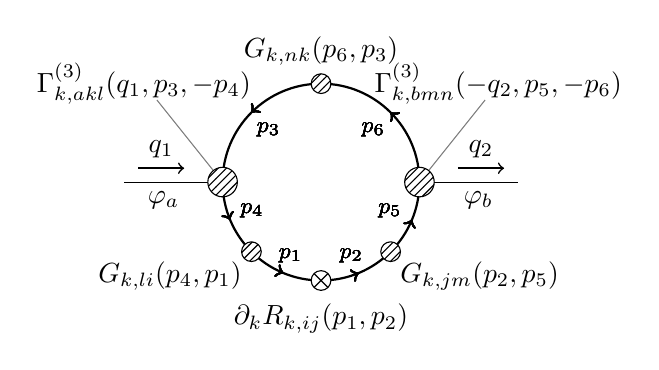
\begin{tikzpicture}
  % Loop
  \draw[loop/.list={{0.0625*2}{6},{0.0625*6}{3},{0.0625*9}{4},{0.0625*11}{1},{0.0625*13}{2},{0.0625*15}{5}}] (0,0) circle (\lrad);
  \draw[cross] (0,-\lrad) circle (\srad) node[below=5pt] {$\partial_k R_{k,ij}(p_1,p_2)$};
  \draw[dressed] (-45:\lrad) circle (\srad) node[below right] {$G_{k,jm}(p_2,p_5)$};
  \draw[dressed] (-135:\lrad) circle (\srad) node[below left] {$G_{k,li}(p_4,p_1)$};
  \draw[dressed] (0,\lrad) circle (\srad) node[above=3pt] {$G_{k,nk}(p_6,p_3)$};

  % External lines
  \draw (-2*\lrad,0) coordinate (xl) -- (-\lrad,0) node[pos=0.4,below] {$\varphi_a$};
  \draw[momentum] (-2*\lrad,0) -- (-1.25*\lrad,0) node[midway,above] {$q_1$};
  \draw (\lrad,0) -- (2*\lrad,0) coordinate (xr) node[pos=0.6,below] {$\varphi_b$};
  \draw[momentum] (1.25*\lrad,0) -- (2*\lrad,0) node[midway,above] {$q_2$};

  % Vertices
  \node at (-1.8*\lrad,\lrad) (Gkail) {$\Gamma_{k,akl}^{(3)}(q_1,p_3,-p_4)$};
  \draw[label] (Gkail) -- (-\lrad,0);
  \draw[dressed] (-\lrad,0) circle (\mrad);
  \node at (1.8*\lrad,\lrad) (Gkbde) {$\Gamma_{k,bmn}^{(3)}(-q_2,p_5,-p_6)$};
  \draw[label] (Gkbde) -- (\lrad,0);
  \draw[dressed] (\lrad,0) circle (\mrad);
\end{tikzpicture}

% Diagram 3
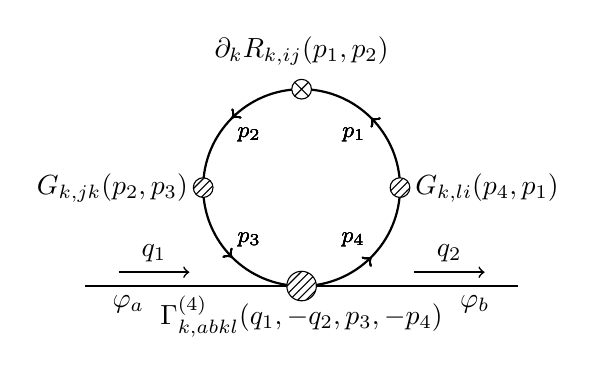
\begin{tikzpicture}
  % Loop
  \draw[loop/.list={{0.0625*2}{1},{0.0625*6}{2},{0.0625*10}{3},{0.0625*14}{4}}] (0,0) circle (\lrad);
  \draw[cross] (0,\lrad) circle (\srad) node[above=5pt] {$\partial_k R_{k,ij}(p_1,p_2)$};
  \draw[dressed] (-\lrad,0) circle (\srad) node[left=2pt] {$G_{k,jk}(p_2,p_3)$};
  \draw[dressed] (\lrad,0) circle (\srad) node[right=2pt] {$G_{k,li}(p_4,p_1)$};

  % External lines
  \draw (-2.2*\lrad,-\lrad) -- (2.2*\lrad,-\lrad) node[pos=0.1,below] {$\varphi_a$} node[pos=0.9,below] {$\varphi_b$};
  \draw[momentum] (-2*\lrad,-\lrad) -- (-\lrad,-\lrad) node[midway,above] {$q_1$};
  \draw[momentum] (\lrad,-\lrad) -- (2*\lrad,-\lrad) node[midway,above] {$q_2$};

  % Vertices
  \draw[dressed] (0,-\lrad) circle (\mrad) node[below] {$\Gamma_{k,abkl}^{(4)}(q_1,-q_2,p_3,-p_4)$};
\end{tikzpicture}

\end{document}
